\documentclass[10pt,a4paper]{article}
\usepackage[utf8]{inputenc}
\usepackage[a4paper, margin=1.4cm, top=1.45cm, bottom=1.45cm]{geometry}
\usepackage{amsmath,amssymb}
\usepackage{xcolor}
\usepackage[most]{tcolorbox}
\usepackage{booktabs}
\usepackage{colortbl}
\usepackage{fancyhdr}
\usepackage{graphicx}
\usepackage{enumitem}
\usepackage{needspace}
\usepackage{array}

% Exact colors from previous lecture notes
\definecolor{themeblue}{rgb}{0.1686, 0.3529, 0.5294}   % #2B5A87
\definecolor{lightbg}{rgb}{0.9098, 0.9333, 0.9569}     % #E8EEF4
\definecolor{accentred}{rgb}{0.7843, 0.2706, 0.2275}   % #C8453A
\definecolor{codebg}{rgb}{0.96, 0.97, 0.98}

% Header and Footer
\pagestyle{fancy}
\fancyhf{}
\fancyhead[L]{\textcolor{themeblue}{\small Lecture 5 --- Logistic Regression}}
\fancyhead[R]{\textcolor{themeblue}{\small Deep Learning}}
\renewcommand{\headrulewidth}{0.5pt}
\renewcommand{\headrule}{\hbox to\headwidth{\color{themeblue}\leaders\hrule height \headrulewidth\hfill}}
\fancyfoot[C]{\thepage}

\begin{document}

% Title Block
\begin{center}
    {\LARGE\bfseries\color{themeblue} Logistic Regression \& Gradient Descent}\\[2pt]
    {\small\itshape Deep Learning (S.-A. Berrani, ENSIA 2026--2027)}\\[2pt]
    \textcolor{themeblue}{\rule{\textwidth}{0.6pt}}
\end{center}

\vspace{-9pt}

% Core Idea & Notation Box
\begin{tcolorbox}[
    colframe=themeblue,
    colback=lightbg,
    coltitle=white,
    fonttitle=\bfseries\sffamily,
    title={Problem Formulation \& Notation},
    arc=1.6mm,
    boxrule=0.6pt,
    left=6pt, right=6pt, top=3pt, bottom=3pt
]
\textbf{Objective:} Predict the probability that a given input sample belongs to a target binary class ($y \in \{0, 1\}$).
\begin{itemize}[leftmargin=12pt, itemsep=1pt, topsep=1pt]
    \item \textbf{Data Instances:} $m$ training examples: $\{(x^{(1)}, y^{(1)}), (x^{(2)}, y^{(2)}), \dots, (x^{(m)}, y^{(m)})\}$.
    \item \textbf{Input Feature Vector:} $x^{(i)} \in \mathbb{R}^{n_x}$ (e.g., unrolled image $32 \times 64 \times 3 = 6144$ pixels).
    \item \textbf{Design Matrix $X$:} $n_x \times m$ matrix with examples as columns: $X = [x^{(1)}, x^{(2)}, \dots, x^{(m)}] \in \mathbb{R}^{n_x \times m}$.
    \item \textbf{Label Vector $Y$:} Row vector of ground-truth labels: $Y = [y^{(1)}, y^{(2)}, \dots, y^{(m)}] \in \mathbb{R}^{1 \times m}$.
    \item \textbf{Model Parameters:} Weight vector $w \in \mathbb{R}^{n_x}$ and scalar bias $b \in \mathbb{R}$.
    \item \textbf{Prediction:} $\hat{y} \in [0, 1]$ (also denoted as activation $a$), representing $\hat{y} = a = P(y = 1 \mid x)$.
\end{itemize}
\end{tcolorbox}

\vspace{1pt}

% Section 1: Definition of y in terms of Probability and w^T x + b
\noindent{\Large\bfseries\color{themeblue} 1. Defining $\hat{y}$ in Terms of Probability and $w^T x + b$}\par\vspace{2pt}
In binary classification, given an input feature vector $x \in \mathbb{R}^{n_x}$, our objective is to predict the conditional probability:
\[
\hat{y} = P(y = 1 \mid x) \in [0, 1] \qquad \implies \qquad P(y = 0 \mid x) = 1 - P(y = 1 \mid x) = 1 - \hat{y}
\]

\begin{itemize}[leftmargin=12pt, itemsep=1.5pt, topsep=1pt]
    \item \textbf{Why a Linear Model Fails:} A linear combination $z = w^T x + b = \sum_{j=1}^{n_x} w_j x_j + b$ spans $(-\infty, +\infty)$. It cannot serve directly as a probability because $z$ can take values $< 0$ or $> 1$, violating probability axioms.
    \item \textbf{The Sigmoid Activation:} To squash $z$ into the valid probability range $(0, 1)$, we apply the \textbf{sigmoid function} $\sigma(z)$:
    \[
    \hat{y} = a = \sigma(z) = \sigma(w^T x + b) = \frac{1}{1 + e^{-(w^T x + b)}}
    \]
    \item \textbf{Asymptotic Behavior:}
    \begin{itemize}[leftmargin=10pt, itemsep=0.5pt]
        \item When $z \to +\infty$: $e^{-z} \to 0 \implies \sigma(z) \to \frac{1}{1 + 0} = \mathbf{1}$ (high confidence in positive class).
        \item When $z \to -\infty$: $e^{-z} \to +\infty \implies \sigma(z) \to \frac{1}{1 + \infty} = \mathbf{0}$ (high confidence in negative class).
        \item When $z = 0$: $\sigma(0) = \frac{1}{1 + 1} = \mathbf{0.5}$ $\implies$ Defines the \textbf{decision boundary} hyperplane $w^T x + b = 0$.
    \end{itemize}
\end{itemize}

\vspace{1pt}

% Section 2: Loss Functions
\noindent{\Large\bfseries\color{themeblue} 2. Loss Functions: Squared Error vs. Binary Cross-Entropy}\par\vspace{2pt}
\textbf{Definition:} The \textbf{loss function} $\mathcal{L}(\hat{y}, y)$ quantifies the error between prediction $\hat{y}$ and label $y$ for a \textbf{single example} $(x, y)$.

\begin{enumerate}[leftmargin=14pt, itemsep=1.5pt, topsep=1pt]
    \item \textbf{Squared Error Loss (MSE for a single instance):}
    $\mathcal{L}_{\text{SE}}(\hat{y}, y) = \frac{1}{2}(\hat{y} - y)^2$.
    \textit{Why avoided for logistic regression?}\\
    (1) \textbf{Non-Convexity:} Substituting $\hat{y} = \sigma(w^T x + b)$ yields a non-convex surface plagued with local minima and saddle points.\\
    (2) \textbf{Vanishing Gradients:} $\frac{\partial \mathcal{L}_{\text{SE}}}{\partial z} = (\hat{y} - y)\sigma'(z) = (\hat{y} - y)\hat{y}(1 - \hat{y})$. If the prediction is confidently wrong ($y = 1$ but $\hat{y} \approx 0$), $\hat{y}(1 - \hat{y}) \approx 0$, so the gradient vanishes and learning halts.

    \item \textbf{Binary Cross-Entropy Loss (Logarithmic Loss / Log Loss):}
    \[
    \mathcal{L}_{\text{BCE}}(\hat{y}, y) = -\big[ y \log \hat{y} + (1 - y) \log(1 - \hat{y}) \big]
    \]
    \begin{itemize}[leftmargin=10pt, itemsep=0.5pt]
        \item \textbf{If $y = 1$:} $\mathcal{L} = -\log(\hat{y})$. As $\hat{y} \to 1$, $\mathcal{L} \to 0$. If $\hat{y} \to 0$, $\mathcal{L} \to +\infty$ (steep penalty).
        \item \textbf{If $y = 0$:} $\mathcal{L} = -\log(1 - \hat{y})$. As $\hat{y} \to 0$, $\mathcal{L} \to 0$. If $\hat{y} \to 1$, $\mathcal{L} \to +\infty$ (steep penalty).
    \end{itemize}
    \textbf{Convexity:} Cross-entropy cancels the $\hat{y}(1 - \hat{y})$ factor during backpropagation, yielding $\frac{\partial \mathcal{L}}{\partial z} = \hat{y} - y$. This ensures the cost function is \textbf{strictly convex} with a unique global minimum.
\end{enumerate}

\vspace{1pt}

\begin{tcolorbox}[
    colframe=accentred,
    colback=white,
    arc=1.5mm,
    boxrule=0.5pt,
    left=6pt, right=6pt, top=2.5pt, bottom=2.5pt
]
\textbf{Brief Note on MLE Derivations:} Both losses arise directly from \textbf{Maximum Likelihood Estimation (MLE)}:
\begin{itemize}[leftmargin=10pt, itemsep=1pt, topsep=1pt]
    \item \textit{Squared Error from MLE:} Derived assuming continuous targets with additive Gaussian noise: $y = w^T x + b + \epsilon$ with $\epsilon \sim \mathcal{N}(0, \sigma^2)$. Maximizing likelihood $\iff$ minimizing negative log-likelihood $\sum \frac{(y - \hat{y})^2}{2\sigma^2} \propto \frac{1}{2}\sum(\hat{y} - y)^2$.
    \item \textit{Binary Cross-Entropy from MLE:} Derived assuming binary labels follow a \textbf{Bernoulli distribution}: $P(y \mid x) = \hat{y}^y (1 - \hat{y})^{1-y}$. Maximizing the joint likelihood $\prod_{i=1}^m P(y^{(i)} \mid x^{(i)})$ is identical to minimizing the negative log-likelihood: $-\sum_{i=1}^m [y^{(i)}\log\hat{y}^{(i)} + (1 - y^{(i)})\log(1 - \hat{y}^{(i)})]$.
\end{itemize}
\end{tcolorbox}

\newpage

% Page 2: Cost Function & Activation Functions
% Section 3: Cost Function
\noindent{\Large\bfseries\color{themeblue} 3. Cost Function: Overall Dataset Objective}\par\vspace{2pt}
\textbf{Definition:} The \textbf{cost function} $J(w, b)$ evaluates global performance over the full training dataset of $m$ examples. It is the arithmetic mean of the loss function across all samples:
\[
J(w, b) = \frac{1}{m} \sum_{i=1}^m \mathcal{L}\big(\hat{y}^{(i)}, y^{(i)}\big)
\]

\begin{itemize}[leftmargin=12pt, itemsep=2pt, topsep=1pt]
    \item \textbf{Cost Function with Cross-Entropy (Logistic Regression):}
    \[
    J(w, b) = -\frac{1}{m} \sum_{i=1}^m \Big[ y^{(i)} \log \hat{y}^{(i)} + (1 - y^{(i)}) \log\big(1 - \hat{y}^{(i)}\big) \Big]
    \]
    Globally convex with respect to $(w, b)$, guaranteeing that gradient descent converges toward the global optimum without getting stuck in local minima.

    \item \textbf{Cost Function with Mean Squared Error (MSE --- Linear Regression):}
    \[
    J(w) = \frac{1}{2m} \sum_{i=1}^m \big(w^T x^{(i)} - y^{(i)}\big)^2 = \frac{1}{2m} \|X^T w - Y\|_2^2
    \]
    \textbf{Analytical Solution vs. Matrix Inversion (Slide 17):} In linear regression, setting $\nabla J = 0$ yields the closed-form normal equation:
    \[
    w^* = (X X^T)^{-1} X Y^T \qquad \text{or} \qquad w^* = (X^T X)^{-1} X^T Y
    \]
    \textit{The Computational Problem:} Inverting an $n_x \times n_x$ matrix incurs $\mathcal{O}(n_x^3)$ complexity. When the feature dimension $n_x$ is large (e.g., $n_x = 6144$ for raw images or millions of features) or if $X^TX$ is non-invertible, analytical inversion is intractable. Hence, iterative \textbf{gradient descent} is essential.
\end{itemize}

\vspace{3pt}

% Section 4: Activation Functions
\noindent{\Large\bfseries\color{themeblue} 4. Activation Functions: Sigmoid vs. Tanh}\par\vspace{2pt}
Neural networks use non-linear activations to model complex relationships. Below is a comparison of Sigmoid and Tanh:

\begin{center}
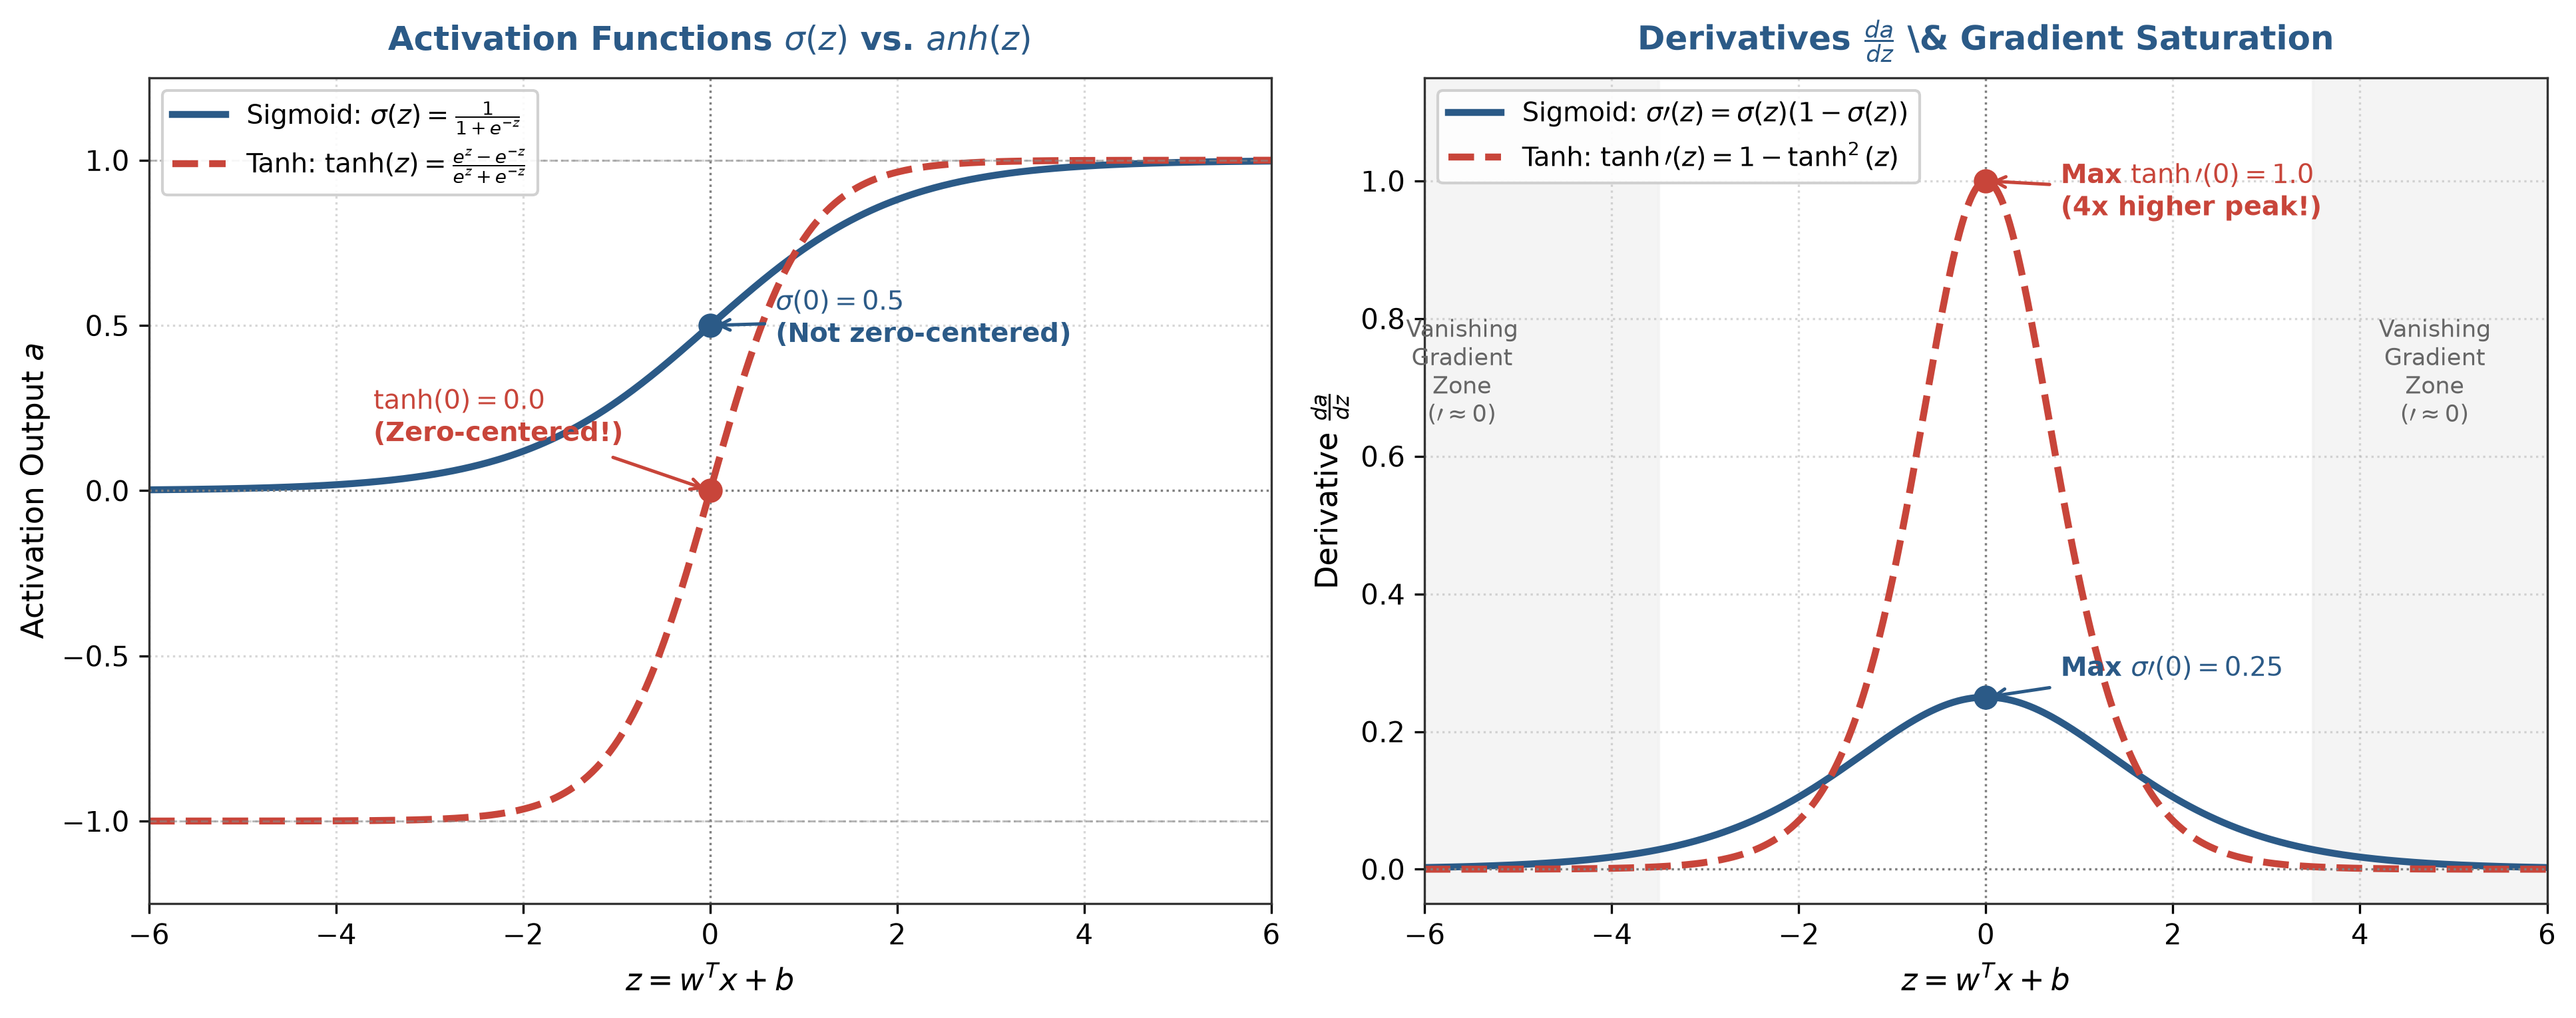
\includegraphics[width=0.84\textwidth]{activation_functions.png}\\[1pt]
{\footnotesize\textit{Comparison of Sigmoid $\sigma(z)$ vs. Tanh $\tanh(z)$ activations and their respective derivatives.}}
\end{center}

\vspace{-4pt}

\begin{center}
\small
\begin{tabular}{>{\raggedright\arraybackslash}p{0.20\textwidth}>{\raggedright\arraybackslash}p{0.36\textwidth}>{\raggedright\arraybackslash}p{0.36\textwidth}}
\toprule
\rowcolor{lightbg}
\textbf{Property} & \textbf{Sigmoid Function $\sigma(z)$} & \textbf{Hyperbolic Tangent $\tanh(z)$} \\
\midrule
\textbf{Mathematical Formula} & $\sigma(z) = \dfrac{1}{1 + e^{-z}}$ & $\tanh(z) = \dfrac{e^z - e^{-z}}{e^z + e^{-z}} = 2\sigma(2z) - 1$ \\
\addlinespace[2pt]
\textbf{Output Range} & $(0, 1)$ & $(-1, 1)$ \\
\addlinespace[2pt]
\textbf{Zero-Centered?} & \textbf{No} ($\sigma(0) = 0.5$) & \textbf{Yes} ($\tanh(0) = 0$) \\
\addlinespace[2pt]
\textbf{Derivative $\frac{da}{dz}$} & $\sigma'(z) = \sigma(z)(1 - \sigma(z))$ & $\tanh'(z) = 1 - \tanh^2(z)$ \\
\addlinespace[2pt]
\textbf{Maximum Derivative} & $\sigma'(0) = 0.25$ & $\tanh'(0) = \mathbf{1.0}$ ($4\times$ larger peak slope) \\
\addlinespace[2pt]
\textbf{Vanishing Gradient} & Severe for $|z| > 4$ ($\sigma'(z) \approx 0$) & Severe for $|z| > 3$ ($\tanh'(z) \approx 0$) \\
\addlinespace[2pt]
\textbf{Primary Role} & Output layer for binary classification & Hidden layers (zero-centered speeds training) \\
\bottomrule
\end{tabular}
\end{center}

\vspace{1pt}
\begin{itemize}[leftmargin=12pt, itemsep=1pt]
    \item \textbf{Why Zero-Centered Matters:} When activations are strictly positive (like Sigmoid), all weight gradients entering a subsequent layer share the same sign, forcing parameters to update in zig-zag trajectories. Because $\tanh(z)$ is zero-centered with mean output near 0, gradients have mixed signs, leading to faster and smoother optimization.
\end{itemize}

\newpage

% Page 3: Fitting the Model, Gradient Descent & Batch Vectorization
% Section 5: Fitting the Model & Gradient Descent
\noindent{\Large\bfseries\color{themeblue} 5. Fitting the Model \& Gradient Descent}\par\vspace{2pt}
\begin{itemize}[leftmargin=12pt, itemsep=2pt]
    \item \textbf{What Does ``Fitting the Model'' Mean?} Fitting (or training) means optimizing the internal parameters $(w, b)$ using the training dataset so that the cost function $J(w, b)$ is minimized:
    \[
    (w^*, b^*) = \arg\min_{w, b} J(w, b)
    \]
    Geometrically, this aligns the decision boundary hyperplane $w^T x + b = 0$ to maximally separate positive examples ($y = 1, \hat{y} > 0.5$) from negative examples ($y = 0, \hat{y} < 0.5$) with high probability.
    \item \textbf{Gradient Descent Update Rule:} An iterative first-order optimization algorithm that starts with an initial parameter guess (e.g., $w = 0, b = 0$) and repeatedly updates parameters in the direction of steepest descent ($-\nabla J$):
    \[
    w := w - \alpha \frac{\partial J(w, b)}{\partial w}, \qquad b := b - \alpha \frac{\partial J(w, b)}{\partial b}
    \]
    where $\alpha > 0$ is the \textbf{learning rate}. If $\alpha$ is too small, learning is slow; if $\alpha$ is too large, the algorithm overshoots and can diverge.
\end{itemize}

\begin{center}
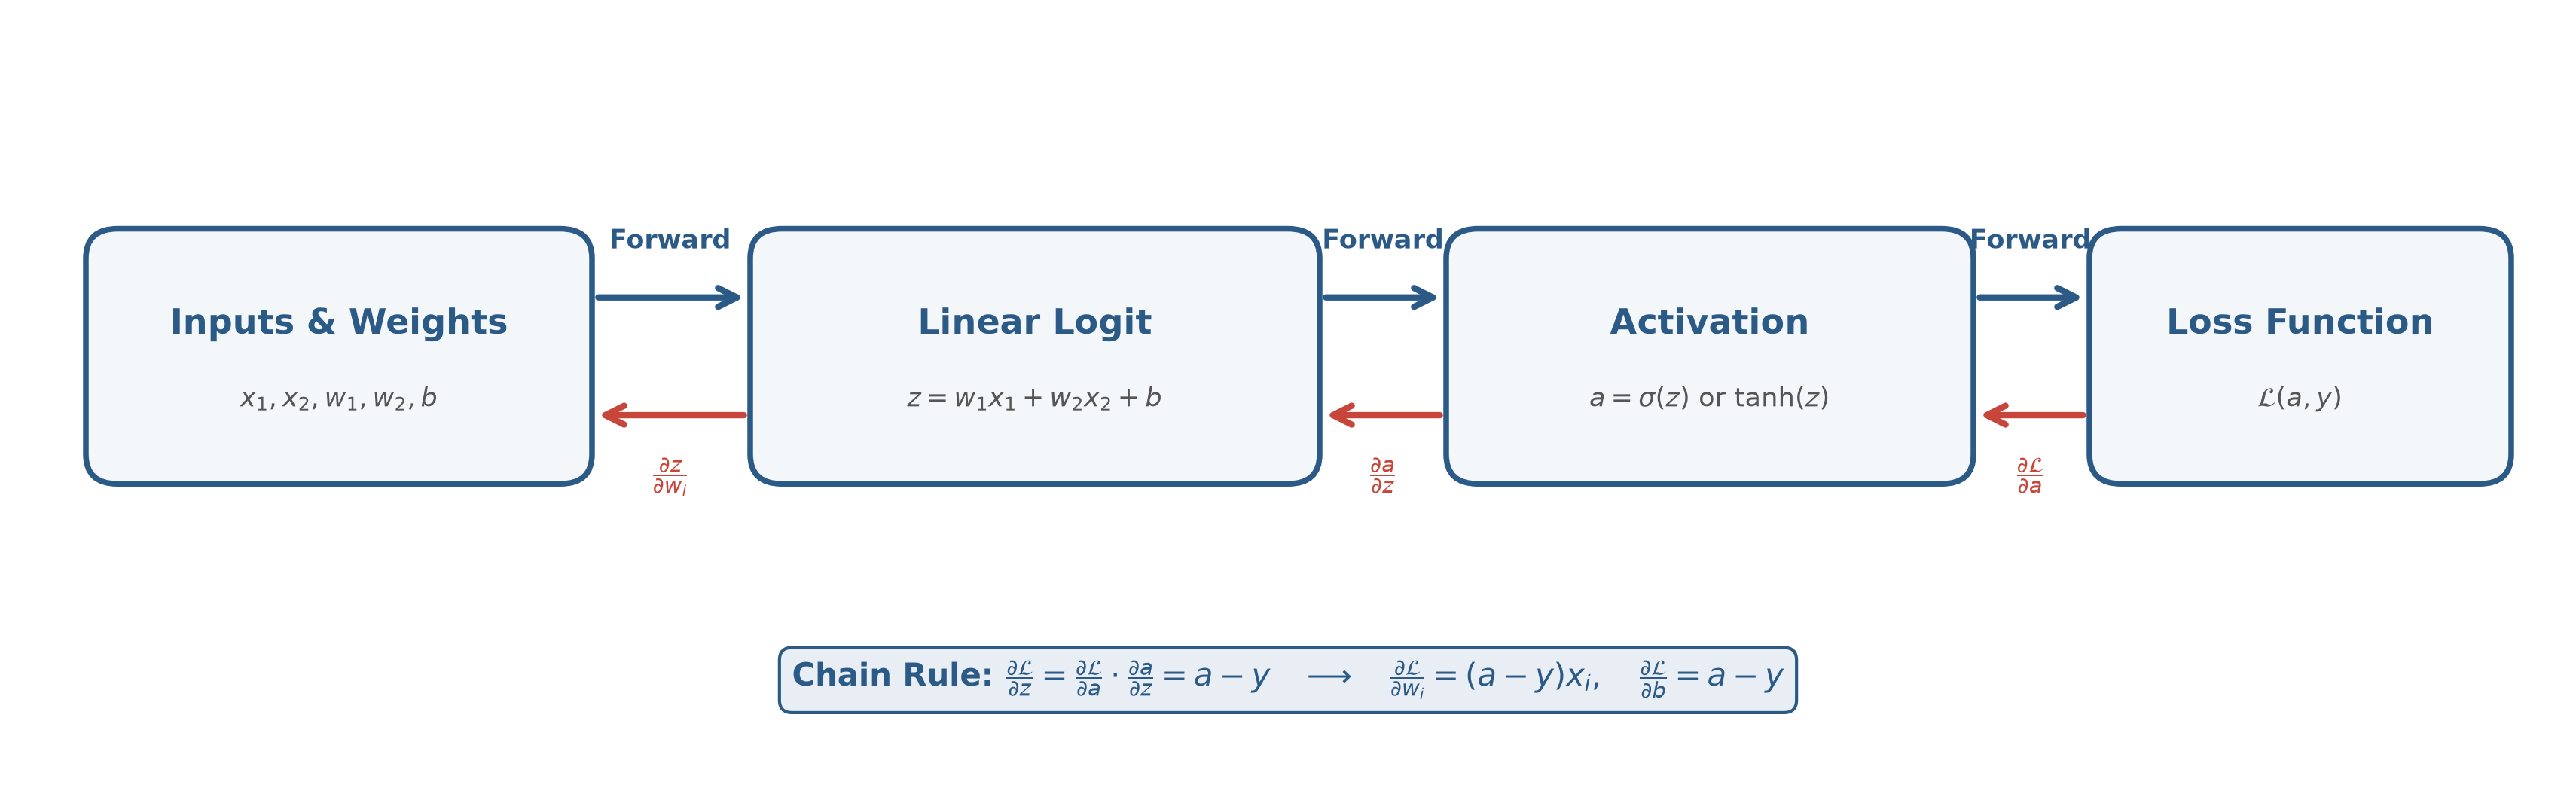
\includegraphics[width=0.82\textwidth]{computation_graph.png}\\[1pt]
{\footnotesize\textit{Computation graph: Forward pass (blue) evaluates logits, activations, and loss; Backward pass (red) computes gradients via the chain rule.}}
\end{center}

\vspace{3pt}

% Section 6: Batch Gradient Descent & Vectorization
\noindent{\Large\bfseries\color{themeblue} 6. Batch Gradient Descent on $m$ Examples \& Vectorization}\par\vspace{2pt}
When computing updates over all $m$ training instances (Slide 25):

\begin{itemize}[leftmargin=12pt, itemsep=2pt]
    \item \textbf{Accumulation Loop Over $m$ Examples:}
    \begin{tcolorbox}[colframe=themeblue, colback=codebg, arc=1.2mm, boxrule=0.4pt, left=6pt, right=6pt, top=2.5pt, bottom=2.5pt]
    \small
    \texttt{J = 0; dw1 = 0; dw2 = 0; db = 0;}\\
    \texttt{for i = 1 to m:}\\
    \hspace*{12pt}\texttt{z(i) = w1*x1(i) + w2*x2(i) + b}\\
    \hspace*{12pt}\texttt{a(i) = sigmoid(z(i))}\\
    \hspace*{12pt}\texttt{J += - (y(i)*log(a(i)) + (1-y(i))*log(1-a(i)))}\\
    \hspace*{12pt}\texttt{dz(i) = a(i) - y(i)}\\
    \hspace*{12pt}\texttt{dw1 += x1(i) * dz(i); \ dw2 += x2(i) * dz(i); \ db += dz(i)}\\
    \texttt{J /= m; dw1 /= m; dw2 /= m; db /= m;}\\
    \texttt{w1 = w1 - alpha * dw1; \ w2 = w2 - alpha * dw2; \ b = b - alpha * db;}
    \end{tcolorbox}

    \item \textbf{Vectorized Formulation (Matrix Equations):}
    Vectorization eliminates explicit loops and accelerates computation using GPU / BLAS operations:
    \begin{align*}
        Z &= w^T X + b \in \mathbb{R}^{1 \times m} \\[2pt]
        A &= \sigma(Z) \in \mathbb{R}^{1 \times m} \\[2pt]
        dZ &= A - Y \in \mathbb{R}^{1 \times m} \\[2pt]
        dw &= \frac{1}{m} X \, dZ^T \in \mathbb{R}^{n_x \times 1}, \qquad db = \frac{1}{m} \sum_{i=1}^m dZ^{(i)} \in \mathbb{R} \\[2pt]
        w &:= w - \alpha \, dw, \qquad b := b - \alpha \, db
    \end{align*}
\end{itemize}

\newpage

% Page 4: Side-by-Side Example Derivation
% Section 7: Side-by-Side Example Derivation
\noindent{\Large\bfseries\color{themeblue} 7. Side-by-Side Example Derivation: $z = w_1 x_1 + w_2 x_2 + b$}\par\vspace{2pt}
Consider a model with 2 input features ($x_1, x_2$), 2 weights ($w_1, w_2$), and bias $b$. Below is the side-by-side comparison of Forward and Backward propagation for:
\begin{itemize}[leftmargin=12pt, itemsep=1pt]
    \item \textbf{Path A:} Sigmoid with Standard Cross-Entropy ($y \in \{0, 1\}$)
    \item \textbf{Path B:} Tanh with Modified Cross-Entropy ($y \in \{-1, +1\}$) \textit{(Slides 26--27)}
\end{itemize}

\vspace{1pt}

\noindent\begin{minipage}[t]{0.485\textwidth}
\begin{tcolorbox}[
    colframe=themeblue, colback=lightbg, coltitle=white,
    fonttitle=\bfseries\sffamily\small,
    title={Path A: Sigmoid + Standard Cross-Entropy},
    arc=1.5mm, boxrule=0.6pt, left=5pt, right=5pt, top=3pt, bottom=3pt
]
\small
\textbf{Label Space:} $y \in \{0, 1\}$\\[2pt]
\textbf{Linear Logit:} $z = w_1 x_1 + w_2 x_2 + b$\\[2pt]
\textbf{Activation:}
\[
a = \sigma(z) = \frac{1}{1 + e^{-z}} \in (0, 1)
\]
\textbf{Loss Function $\mathcal{L}(a, y)$:}
\[
\mathcal{L} = -\big[ y \log a + (1 - y) \log(1 - a) \big]
\]
\hrulefill\\[2pt]
\textbf{Backward Step 1: $\frac{\partial \mathcal{L}}{\partial a}$}
\[
\frac{\partial \mathcal{L}}{\partial a} = -\frac{y}{a} + \frac{1 - y}{1 - a} = \frac{a - y}{a(1 - a)}
\]
\textbf{Backward Step 2: $\frac{\partial a}{\partial z}$}
\[
\frac{\partial a}{\partial z} = \sigma'(z) = a(1 - a)
\]
\textbf{Backward Step 3: $\frac{\partial \mathcal{L}}{\partial z}$ (Chain Rule)}
\[
\frac{\partial \mathcal{L}}{\partial z} = \frac{\partial \mathcal{L}}{\partial a} \cdot \frac{\partial a}{\partial z} = \frac{a - y}{a(1 - a)} \cdot a(1 - a) = \mathbf{a - y}
\]
\textbf{Backward Step 4: Gradients w.r.t Parameters}
\[
\frac{\partial \mathcal{L}}{\partial w_1} = \frac{\partial \mathcal{L}}{\partial z} \frac{\partial z}{\partial w_1} = (a - y) \, x_1
\]
\[
\frac{\partial \mathcal{L}}{\partial w_2} = \frac{\partial \mathcal{L}}{\partial z} \frac{\partial z}{\partial w_2} = (a - y) \, x_2
\]
\[
\frac{\partial \mathcal{L}}{\partial b} = \frac{\partial \mathcal{L}}{\partial z} \frac{\partial z}{\partial b} = a - y
\]
\textbf{Parameter Update Rules:}
\[
w_1 := w_1 - \alpha (a - y) x_1
\]
\[
w_2 := w_2 - \alpha (a - y) x_2
\]
\[
b := b - \alpha (a - y)
\]
\end{tcolorbox}
\end{minipage}
\hfill
\begin{minipage}[t]{0.485\textwidth}
\begin{tcolorbox}[
    colframe=accentred, colback=white, coltitle=white,
    fonttitle=\bfseries\sffamily\small,
    title={Path B: Tanh + Modified Cross-Entropy},
    arc=1.5mm, boxrule=0.6pt, left=5pt, right=5pt, top=3pt, bottom=3pt
]
\small
\textbf{Label Space:} $y \in \{-1, +1\}$\\[2pt]
\textbf{Linear Logit:} $z = w_1 x_1 + w_2 x_2 + b$\\[2pt]
\textbf{Activation:}
\[
a = \tanh(z) = \frac{e^z - e^{-z}}{e^z + e^{-z}} \in (-1, 1)
\]
\textbf{Modified Loss $\mathcal{L}(a, y)$ (Slides 26--27):}
\[
\mathcal{L} = -\left[ \frac{1+y}{2} \log\left(\frac{1+a}{2}\right) + \frac{1-y}{2} \log\left(\frac{1-a}{2}\right) \right]
\]
\hrulefill\\[2pt]
\textbf{Backward Step 1: $\frac{\partial \mathcal{L}}{\partial a}$}
\[
\frac{\partial \mathcal{L}}{\partial a} = -\frac{1+y}{2(1+a)} + \frac{1-y}{2(1-a)} = \mathbf{\frac{a - y}{1 - a^2}}
\]
\textbf{Backward Step 2: $\frac{\partial a}{\partial z}$}
\[
\frac{\partial a}{\partial z} = \tanh'(z) = 1 - a^2
\]
\textbf{Backward Step 3: $\frac{\partial \mathcal{L}}{\partial z}$ (Chain Rule)}
\[
\frac{\partial \mathcal{L}}{\partial z} = \frac{\partial \mathcal{L}}{\partial a} \cdot \frac{\partial a}{\partial z} = \frac{a - y}{1 - a^2} \cdot (1 - a^2) = \mathbf{a - y}
\]
\textbf{Backward Step 4: Gradients w.r.t Parameters}
\[
\frac{\partial \mathcal{L}}{\partial w_1} = \frac{\partial \mathcal{L}}{\partial z} \frac{\partial z}{\partial w_1} = (a - y) \, x_1
\]
\[
\frac{\partial \mathcal{L}}{\partial w_2} = \frac{\partial \mathcal{L}}{\partial z} \frac{\partial z}{\partial w_2} = (a - y) \, x_2
\]
\[
\frac{\partial \mathcal{L}}{\partial b} = \frac{\partial \mathcal{L}}{\partial z} \frac{\partial z}{\partial b} = a - y
\]
\textbf{Parameter Update Rules:}
\[
w_1 := w_1 - \alpha (a - y) x_1
\]
\[
w_2 := w_2 - \alpha (a - y) x_2
\]
\[
b := b - \alpha (a - y)
\]
\end{tcolorbox}
\end{minipage}

\vspace{3pt}

\begin{tcolorbox}[
    colframe=themeblue, colback=lightbg, arc=1.5mm, boxrule=0.5pt,
    left=7pt, right=7pt, top=3pt, bottom=3pt
]
\textbf{Mathematical Symmetry Insight:} In both architectures, the denominator of the loss gradient exactly cancels the derivative of the activation function:
\[
\text{Sigmoid: } \frac{a - y}{a(1 - a)} \cdot a(1 - a) = a - y \qquad\Big\vert\qquad \text{Tanh: } \frac{a - y}{1 - a^2} \cdot (1 - a^2) = a - y
\]
This demonstrates that the modified cross-entropy loss was specifically designed so that Tanh preserves the clean, error-proportional gradient flow $a - y$.
\end{tcolorbox}

\end{document}
